%%%%%%%%%%%%%%%%%%%%%%%%%%%%%%%%%%%%%%%%%%%%%%%%%%%%%%%%%%%%%%%%%%
\section{Leaflet driven by a sinusoidal channel flow}
\label{sec:leaflet}
%%%%%%%%%%%%%%%%%%%%%%%%%%%%%%%%%%%%%%%%%%%%%%%%%%%%%%%%%%%%%%%%%%

\noindent
The second benchmark exercises the coupling under strong time-dependent forcing. A thin flexible leaflet, clamped along one edge, oscillates in response to a periodic channel flow whose direction reverses every half-period. The configuration is taken from the immersed finite element method (IFEM) study of \citet{zhang_immersed_2007}, where it serves as the canonical FSI verification case, and it has since been used by several groups developing related immersed and fictitious-domain formulations \citep{baaijens_fictitiousdomain_2001,de_hart_threedimensional_2003,zhang_immersed_2012,roy_benchmarking_2015}. The geometry is idealised, but the combination of strong unsteady forcing, large structural rotation, and bidirectional loading makes it a stringent test of whether an FSI scheme transfers momentum and kinematic information consistently across the interface.

\noindent
In the original study the leaflet is a two-dimensional nearly incompressible hyperelastic continuum discretised by quadrilateral finite elements and immersed in a non-conforming Eulerian finite element fluid mesh. The two are coupled through a smoothed Dirac-delta-like interpolation operator that both spreads the interaction forces to the fluid and interpolates the fluid velocity onto the solid, which generalises Peskin's immersed boundary method \citep{peskin_immersed_2002} by removing the assumption of a fibre-like solid and the requirement of a uniform background mesh \citep{de_hart_threedimensional_2003}. The leaflet response is fully resolved as a two-dimensional continuum, including through-thickness stretching and shearing and the surrounding tractions on its faces. The present approach instead reduces the structure to a slender Simo--Reissner beam whose centreline coincides with the leaflet mid-line, with the rectangular cross-section entering only through its inertia and bending stiffness, and couples it through the actuator-line operators of Section~\ref{sec:almCouplingTheory}. The leaflet therefore exerts a force on the fluid without occupying a discrete volume in the CFD mesh, and the channel mesh remains static. The framework is lighter, but it assumes the leaflet is loaded by quasi-steady normal drag rather than by resolved surface tractions, and whether that assumption holds in the oscillatory low-Reynolds regime is what the benchmark assesses.

\subsection{Problem definition}
\label{sec:leaflet_geometry}
The geometry is presented in Figure~\ref{fig:leaflet_schematic} and follows \citet{zhang_immersed_2007}, Section~3.2. The fluid domain is a rectangular channel of length $L = 4~\mathrm{cm}$ and full width $2H = 2~\mathrm{cm}$, with the origin where the inlet plane meets the channel mid-plane. The leaflet is a thin flexible body of length $\lambda = 0.8~\mathrm{cm}$ and thickness $t_{\ell} = 0.0212~\mathrm{cm}$, where the subscript distinguishes it from the time $t$, clamped at the mid-length of the channel and free at the other end. The clamped end is anchored on the channel mid-plane, so only one half of the original domain is simulated, with the mid-plane treated as a symmetry boundary carrying the leaflet root and a simulated transverse extent of $H = 1~\mathrm{cm}$. As in Section~\ref{sec:beamtunnel}, the problem is solved on a three-dimensional fluid mesh one cell thick in the spanwise direction $z$, here of depth $t_{\ell}$, with symmetry conditions on the two faces normal to $z$, so the flow does not vary across the span while the beam keeps its physical cross-section.

\begin{figure}[!ht]
\centering
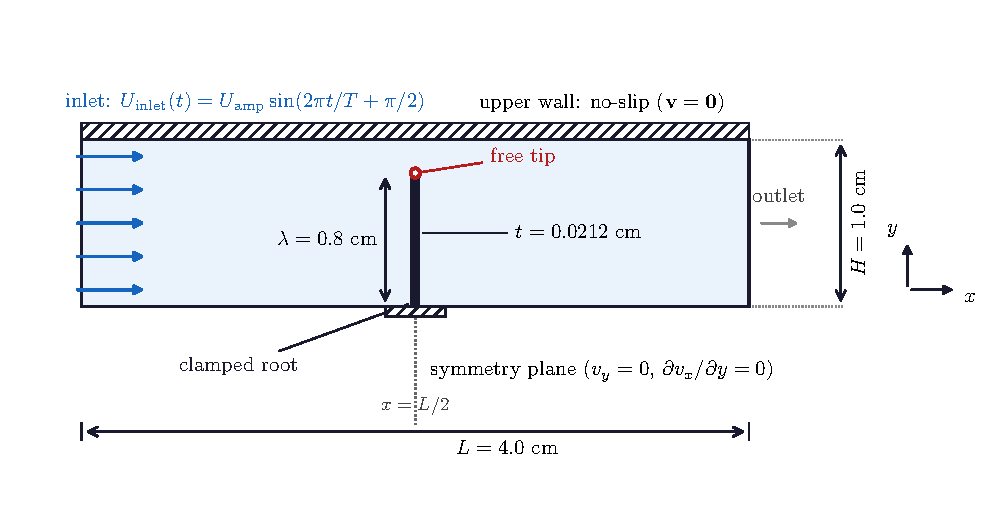
\includegraphics[width=0.88\textwidth]{leaflet_schematic.pdf}
\caption{The leaflet-in-channel verification problem, drawn as the simulated half-domain. The leaflet, of length $\lambda$ and thickness $t_{\ell}$, is clamped at the channel mid-plane at $x = L/2$ and free at its tip. A sinusoidal channel flow is imposed at the inlet, the opposite wall is no-slip, and the lower edge is a symmetry boundary. Dimensions reproduce \citet{zhang_immersed_2007}, Section~3.2.}
\label{fig:leaflet_schematic}
\end{figure}

\noindent
A spatially uniform, time-periodic horizontal velocity is prescribed at the inlet,
\begin{equation}
U_{\mathrm{inlet}}(t) = U_{\mathrm{amp}} \sin\!\left(\frac{2\pi t}{T} + \frac{\pi}{2}\right),
\label{eq:leaflet_inlet}
\end{equation}
so the flow begins at its peak amplitude, the phase shift being chosen for consistency with the original paper in which the leaflet is released from rest into a fully developed inflow. The downstream boundary is an outflow with a fixed reference pressure and zero normal gradient of velocity, the upper boundary a stationary no-slip wall, and the lower boundary a symmetry plane that simultaneously models the channel mid-plane and anchors the leaflet root. Both the fluid and the leaflet start at rest with the leaflet undeformed.

\noindent
The fluid is a Newtonian incompressible liquid of density $10^{3}~\mathrm{kg\,m^{-3}}$, and the leaflet has density $\rho_{s} = 6\times10^{3}~\mathrm{kg\,m^{-3}}$, Young's modulus $E = 10^{6}~\mathrm{Pa}$, and Poisson ratio $\nu = 0.5$. In the present beam formulation the Poisson ratio enters only through the shear modulus $G = E/[2(1+\nu)]$, evaluated at the reference value for consistency with the original constitutive description. The regime is characterised by a Reynolds number $\mathrm{Re} = \rho\,U_{\mathrm{amp}}\,H / \mu$ and a Strouhal number $\mathrm{St} = H / (U_{\mathrm{amp}}\,T)$, defined as in the reference paper. The four combinations used here are listed in Table~\ref{tab:leaflet_cases}.

\begin{table}[!ht]
\centering
\small
\caption{Forcing parameters for the four (Re, St) cases of \citet{zhang_immersed_2007}, Section~3.2, with the cross-section Reynolds and Keulegan--Carpenter numbers $\mathrm{Re}_{t} = \rho\,U_{\mathrm{amp}}\,t_{\ell}/\mu$ and $\mathrm{KC} = U_{\mathrm{amp}}\,T/t_{\ell}$. All cases share $\rho = 10^{3}~\mathrm{kg\,m^{-3}}$, $H = 10^{-2}~\mathrm{m}$, and $t_{\ell} = 2.12\times10^{-4}~\mathrm{m}$. The last column is the normal drag coefficient passed to the closure, taken from the rigid-plate channel calibration of Section~\ref{sec:leaflet_cd_calibration} at each case's own Reynolds number.}
\label{tab:leaflet_cases}
\setlength{\tabcolsep}{6pt}
\renewcommand{\arraystretch}{1.15}
\begin{tabular}{c c c c c c c c}
\toprule
Case & $U_{\mathrm{amp}}$ (m\,s$^{-1}$) & $T$ (s) & $\mu$ (Pa\,s) & $\mathrm{Re}$ & $\mathrm{St}$ & $\mathrm{KC}$ & $C_{dn}$ \\
\midrule
C1 & $0.01$ & $1$ & $10^{-2}$ & $10$ & $1.0$ & $47$ & $108$ \\
C2 & $0.01$ & $1$ & $10^{-1}$ & $1$  & $1.0$ & $47$ & $332$ \\
C3 & $0.01$ & $2$ & $10^{-1}$ & $1$  & $0.5$ & $94$ & $332$ \\
C4 & $0.01$ & $2$ & $10^{-2}$ & $10$ & $0.5$ & $94$ & $108$ \\
\bottomrule
\end{tabular}
\end{table}

\subsection{Steady-CFD calibration of the normal drag coefficient}
\label{sec:leaflet_cd_calibration}

\noindent
As in Section~\ref{sec:beamtunnel_cd_calibration}, $C_{dn}$ must reflect the drag that would act on a rigid leaflet of the same cross-section in the same channel at the same Reynolds number. Two steady-CFD setups are used, illustrated in Figure~\ref{fig:leaflet_dragCalib_mesh}. The first is an unbounded cross-section calibration, which measures the free-stream drag $C_{d}^{\infty}$ of the leaflet cross-section in isolation. The second is a rigid-plate channel calibration, which measures the in-channel drag $C_{d}$ of the full leaflet in the coupled domain. Both are solved as steady flows with the SIMPLE algorithm, as implemented in the \texttt{simpleFoam} solver of OpenFOAM. The meshes are generated by octree-based splitting of a hexahedral background mesh around the plate surface, as implemented in the \texttt{snappyHexMesh} utility of OpenFOAM, where each refinement level halves the cell size. Three levels are applied in a zone enveloping the plate and four to five on the plate surface, giving a smallest cell at the plate of $1.3\times10^{-5}~\mathrm{m}$ and $8\times10^{-6}~\mathrm{m}$ respectively. The channel calibration uses the same $150\times38$ background mesh as the coupled simulation, which removes any mesh-related component of the discrepancy between the calibration result and the value seen by the closure at run time.

\begin{figure}[!ht]
\centering
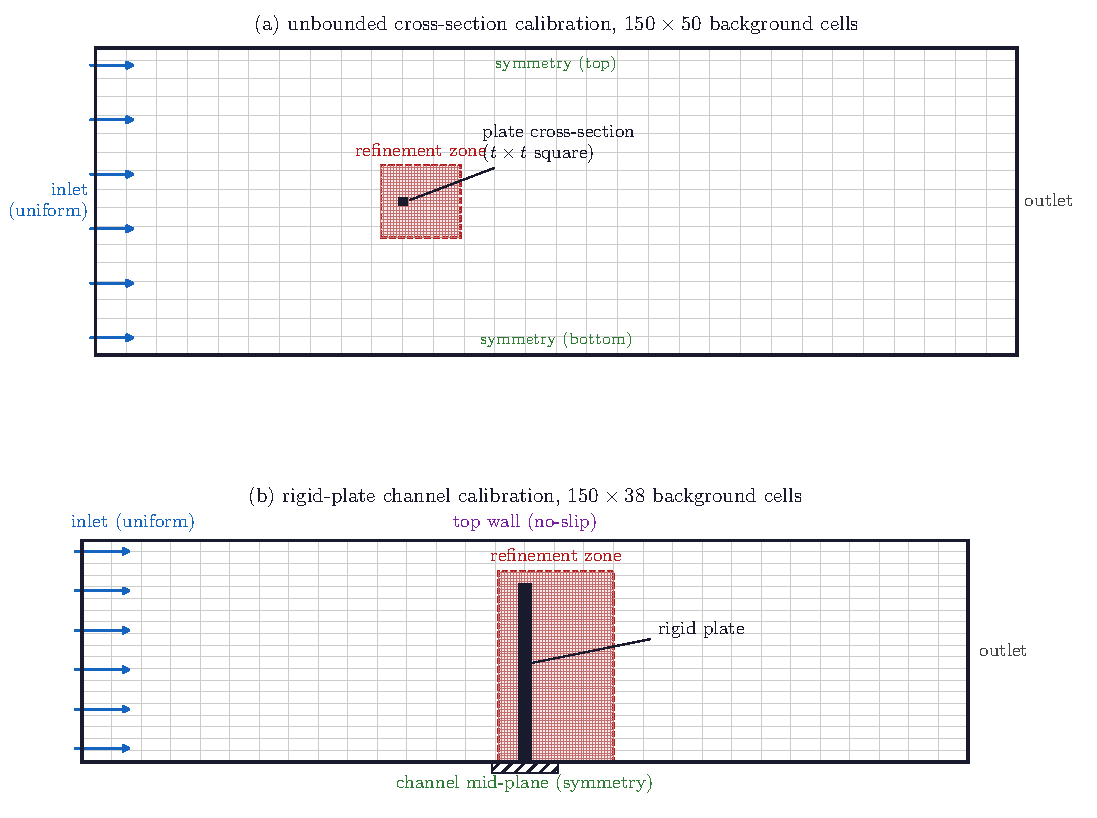
\includegraphics[width=0.88\textwidth]{leaflet_dragCalib_mesh.pdf}
\caption{The two steady-CFD drag-calibration setups. (a) Unbounded cross-section in plan view, with the square cross-section of side $t_{\ell}$ in an unbounded stream, symmetry on the two lateral boundaries and on the two faces that bound the thin domain along the plate axis, returning the free-stream drag ($A_{\mathrm{ref}} = t_{\ell}^{2}$). (b) Rigid-plate channel, with a rigid plate of length $\lambda$ and thickness $t_{\ell}$ in the coupled channel, the mid-plane treated as a symmetry plane and the opposite wall as no-slip, returning the in-channel drag ($A_{\mathrm{ref}} = t_{\ell}\,\lambda$). A local refinement zone is shown in red.}
\label{fig:leaflet_dragCalib_mesh}
\end{figure}

\noindent
The unbounded configuration has four boundaries parallel to the flow, namely the two lateral boundaries drawn at the top and bottom of Figure~\ref{fig:leaflet_dragCalib_mesh}(a) and the two faces normal to the plate axis, which bound the thin domain above and below the plane of that drawing. All four are symmetry planes. The symmetry on the two faces normal to the plate axis makes the cross-section behave as an infinitely long cylinder, so the case is equivalent to a two-dimensional one. Figure~\ref{fig:leaflet_dragCalib}(a) shows the trace decreasing monotonically to $C_{d}^{\infty} \approx 36.8$ at the C1 cross-section Reynolds number $\mathrm{Re}_{t} = 0.212$, between the Oseen estimate \citep{lamb_hydrodynamics_1932} for a low-Reynolds two-dimensional cylinder ($\approx 25$) and the empirical estimate of \citet{hoerner_fluid_1965} for a flat-plate cross-section ($\approx 50$). This is not the coefficient passed to the closure, because the leaflet sits in a channel of half-width $H = 10\,t_{\ell}$ where the blockage and the walls modify the drag. Its role is a literature-comparable check on the cross-section drag and a baseline for the confinement amplification.

\noindent
In the channel configuration the lower boundary is the channel mid-plane and is treated as a symmetry plane, because reflecting the half-domain across it recovers a plate floating freely at the centreline of a full channel of width $2H$, which is the reference geometry. Figure~\ref{fig:leaflet_dragCalib}(b) shows the in-channel coefficient converging to $C_{d} \approx 108$ at $\mathrm{Re} = 10$, almost three times the unbounded value. That ratio of $2.9$ quantifies the cumulative effect of blockage, aspect ratio, and viscous coupling along the full plate length, and decomposing the force shows that pressure accounts for approximately $98\%$ of the total, so the in-channel drag is dominated by upstream stagnation and leeward suction. At $\mathrm{Re} = 1$ the same calibration gives $C_{d} \approx 332$, about three times larger, reflecting the thickening of the viscous boundary layer around the plate, which effectively enlarges the bluff cross-section and raises the upstream-face pressure rise. A single calibration cannot therefore be transferred between the two Reynolds numbers, and each coupled case uses the value calibrated at its own. This is a real limitation of the closure, since a coefficient that has to be re-established whenever the Reynolds number or the blockage changes restricts where the method can be applied without a preparatory run. The value passed to the closure is the in-channel coefficient at the matching Reynolds number, identified with the closure input through $C_{dn} = C_{d}$ as checked in Section~\ref{sec:leaflet_probe}, and the tangential coefficient is fixed at $C_{dt} = 0.01$ as before.

\begin{figure}[!ht]
\centering
\begin{subfigure}[b]{0.48\textwidth}
  \centering
  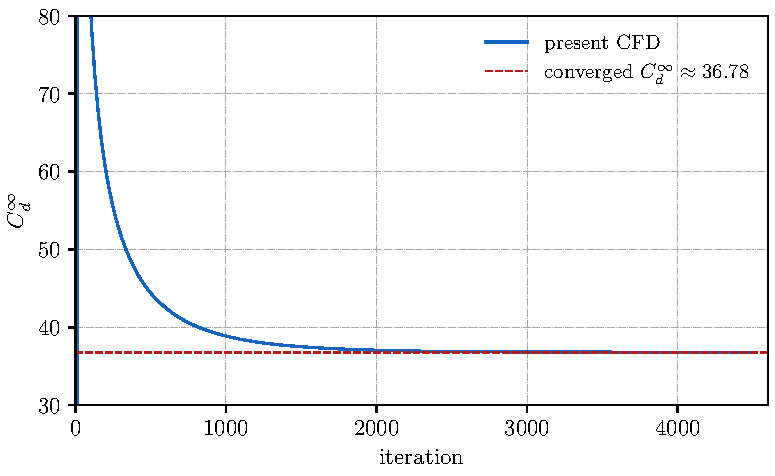
\includegraphics[width=\linewidth]{leaflet_dragCalib_topview.pdf}
  \caption{}
\end{subfigure}\hfill
\begin{subfigure}[b]{0.48\textwidth}
  \centering
  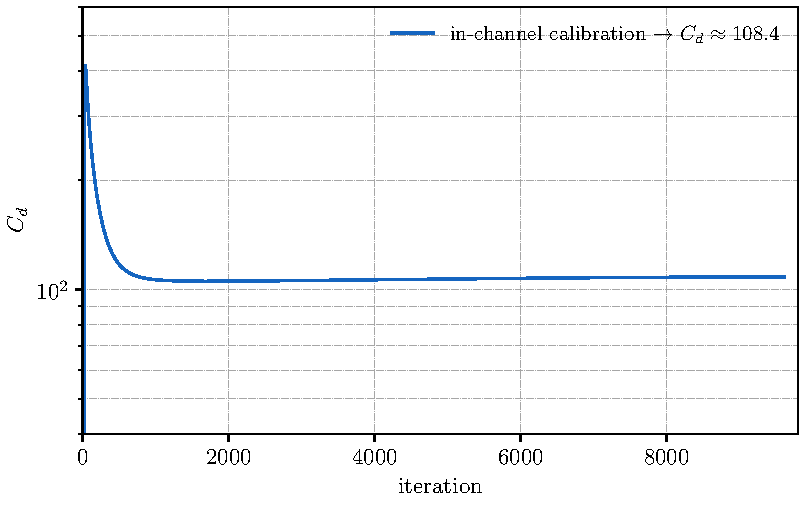
\includegraphics[width=\linewidth]{leaflet_dragCalib_sideview_paper.pdf}
  \caption{}
\end{subfigure}
\caption{Convergence of the two steady-CFD drag calibrations. (a) Free-stream drag coefficient for the unbounded cross-section at $\mathrm{Re}_{t} = 0.212$, converging to $36.8$. (b) In-channel drag coefficient at $\mathrm{Re} = 10$, converging to $C_{d} \approx 108$.}
\label{fig:leaflet_dragCalib}
\end{figure}

\subsection{Check of the identification $C_{dn} = C_{d}$}
\label{sec:leaflet_probe}

\noindent
Identifying $C_{dn}$ with $C_{d}$ is not automatic, because the two are normalised by different velocities. This subsection checks whether the coefficient calibrated in Section~\ref{sec:leaflet_cd_calibration} can be passed to the closure unchanged. The check samples the converged channel calibration and uses no new configuration, so it verifies the calibration rather than adding a second one. At each beam node the closure samples the local fluid velocity $U_{s}$ at the fixed offset $r_{s} = 3.18\times10^{-3}~\mathrm{m}$ upstream of the node and applies a normal load per unit length of $\tfrac{1}{2}\rho\,C_{dn}\,t_{\ell}\,U_{s}^{2}$, whereas the steady CFD normalises the integrated rigid-plate drag by the channel inlet velocity, giving an equivalent force per unit length of $\tfrac{1}{2}\rho\,C_{d}\,t_{\ell}\,U_{\mathrm{in}}^{2}$ averaged over the plate length. Requiring the two to apply the same force per unit length on average along the beam, so that the calibration carries unchanged into the coupled run, gives
\begin{equation}
\label{eq:cdn_correction}
C_{dn} \;=\; C_{d}\,
\frac{U_{\mathrm{in}}^{2}}{\langle U_{s}^{2}\rangle_{\mathrm{beam}}},
\qquad
\langle U_{s}^{2}\rangle_{\mathrm{beam}} \;\equiv\; \frac{1}{\lambda}\int_{0}^{\lambda} U_{s}^{2}(y)\,\mathrm{d}y,
\end{equation}
so the identification is exact if and only if the beam-averaged squared sampled velocity equals the inlet squared velocity.

\noindent
To check the condition, the converged $\mathrm{Re} = 10$ channel calibration is sampled along a line at $x = L/2 - r_{s}$, with the streamwise velocity extracted at $81$ uniformly spaced points spanning the beam. Squaring the profile and applying Eq.~\eqref{eq:cdn_correction} gives $\langle U_{s}^{2}\rangle_{\mathrm{beam}}/U_{\mathrm{in}}^{2} = 1.006$. Figure~\ref{fig:leaflet_probe_profile} shows why. The curve varies strongly along the beam, reduced to $0.24$ at the root where the plate stagnation slows the flow and rising to $3.36$ at the tip where the fluid accelerates through the narrow gap to the opposite wall, but the two departures balance almost exactly, so the average sits within $0.6\%$ of the reference and the correction can be dropped.

\begin{figure}[!ht]
\centering
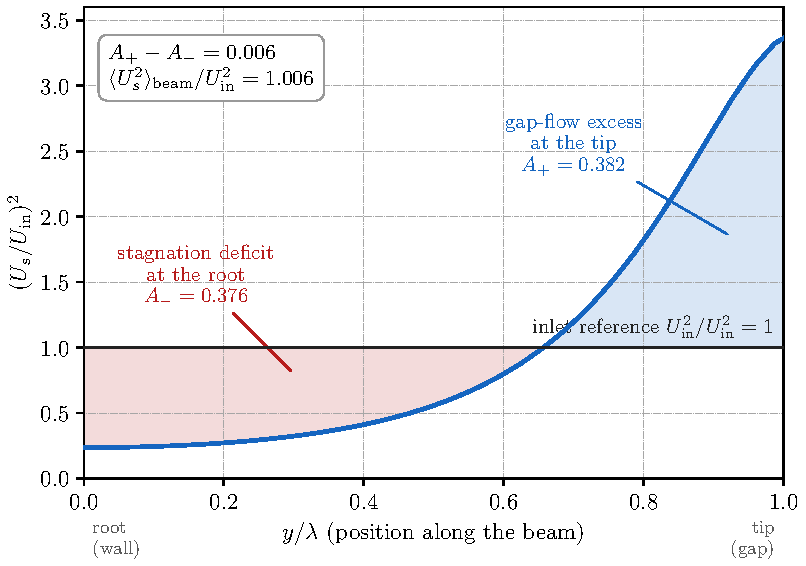
\includegraphics[width=0.72\textwidth]{leaflet_probe_profile.pdf}
\caption{Squared sampled velocity $(U_{s}/U_{\mathrm{in}})^{2}$ along the beam at the upstream-sampling line, in the converged $\mathrm{Re} = 10$ channel calibration. For $C_{dn} = C_{d}$ to hold exactly, the beam average must equal the inlet reference (horizontal line). The deficit area below the reference near the root ($A_- = 0.376$) is cancelled almost exactly by the excess above it near the tip ($A_+ = 0.382$), leaving the beam average at $1.006$.}
\label{fig:leaflet_probe_profile}
\end{figure}

\noindent
That the two nearly cancel is specific to this geometry. Without the plate, the sampling line would lie in the undisturbed fully developed channel flow, whose Poiseuille profile peaks at $1.5\,U_{\mathrm{in}}$ on the symmetry plane and integrates to $1.474$, so a leaflet in undisturbed flow would see a $47\%$ enhancement of the squared driving velocity and the correction could not be dropped. The actual plate blocks $80\%$ of the channel half-width, so most of the upstream flow either stagnates near the root or accelerates through the tip gap, which redistributes the squared profile sharply away from the parabolic shape. In a less confined channel the same probe-line analysis would return a value distinctly above unity and the explicit correction would have to be retained.

\subsection{Time step and flow snapshots}
\label{sec:leaflet_snapshots}

\noindent
The temporal resolution is selected from a study on case C1, in which four time steps spanning a factor of twenty are run to statistical convergence with all other inputs held fixed (Figure~\ref{fig:leaflet_dt_study}). The two finest steps collapse onto a common trace, with half-amplitudes of $2.324~\mathrm{mm}$ at $\Delta t = 5\times10^{-5}~\mathrm{s}$ and $2.355~\mathrm{mm}$ at $10^{-4}~\mathrm{s}$, a difference of $1.3\%$ and no visible phase drift over the two reported periods. The two coarser steps under-predict the response, giving $2.036~\mathrm{mm}$ at $2.5\times10^{-4}~\mathrm{s}$ and $2.084~\mathrm{mm}$ at $10^{-3}~\mathrm{s}$, so the coarsest step gives the larger of the two values. The four steps are not related by a constant refinement ratio, the successive reductions being by factors of $4$, $2.5$, and $2$, so they are not used to estimate an order of convergence. The non-monotonic ordering of the two coarser values indicates that at time steps of $2.5\times10^{-4}~\mathrm{s}$ and larger the explicit sampling and quasi-steady closure are no longer integrated with sufficient resolution to track the half-cycle build-up of tip excursion. The finest setting is adopted for all four cases, so that the same step is shared by the higher-$\mathrm{KC}$ cases C3 and C4 without further verification.

\begin{figure}[!ht]
\centering
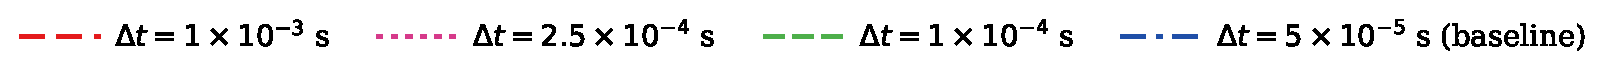
\includegraphics[width=0.90\textwidth]{leaflet_dtStudyLegend.pdf}\\[0.3em]
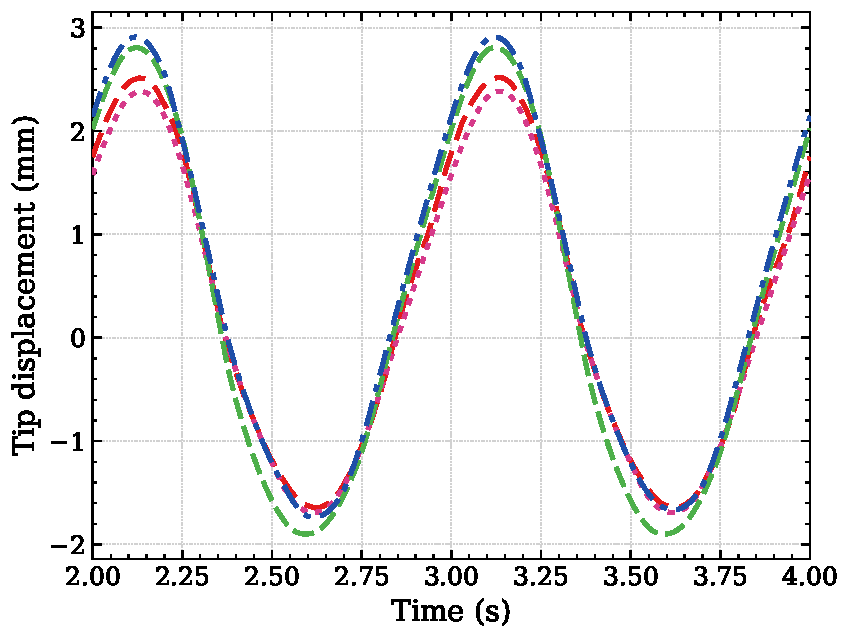
\includegraphics[width=0.68\textwidth]{leaflet_dtStudy.pdf}
\caption{Time-step convergence of the leaflet tip horizontal displacement for case C1 ($\mathrm{Re} = 10$, $\mathrm{St} = 1$), over the converged window $t \in [2, 4]~\mathrm{s}$, with $\Delta t = 5\times10^{-5}~\mathrm{s}$ taken as the converged reference.}
\label{fig:leaflet_dt_study}
\end{figure}

\noindent
Figure~\ref{fig:leaflet_snapshots_panel} shows the converged field over the first half of a forcing period of case C1, at intervals of $T/8$, with the in-plane streamlines coloured by kinematic pressure and the deflected actuator line overlaid in red. The second half of the period is the mirror image of the first and is not reproduced. Because the imposed inlet signal of Eq.~\eqref{eq:leaflet_inlet} carries a $+\pi/2$ phase shift, the velocity extrema fall at $t = 0$ and $T/2$ and the zero crossings at $T/4$ and $3T/4$. At $t = 0$ the leaflet attains its instantaneous maximum tip excursion and a clear pressure dipole develops across the line, with a stagnation patch on the upstream face and a suction patch on the downstream face that switch sides at the opposite extremum. At $T/4$ the streamlines straighten out as the bulk flow reverses and the pressure field is comparatively uniform. The small recirculation pair that lingers near the deflected leaflet at that phase is the residual of the previous half-cycle wake, which confirms that the quasi-steady closure generates no wake of its own, only the redistribution of the resolved field around the moving line of momentum sinks.

\begin{figure}[!ht]
\centering
\begin{subfigure}[b]{0.48\textwidth}
\centering
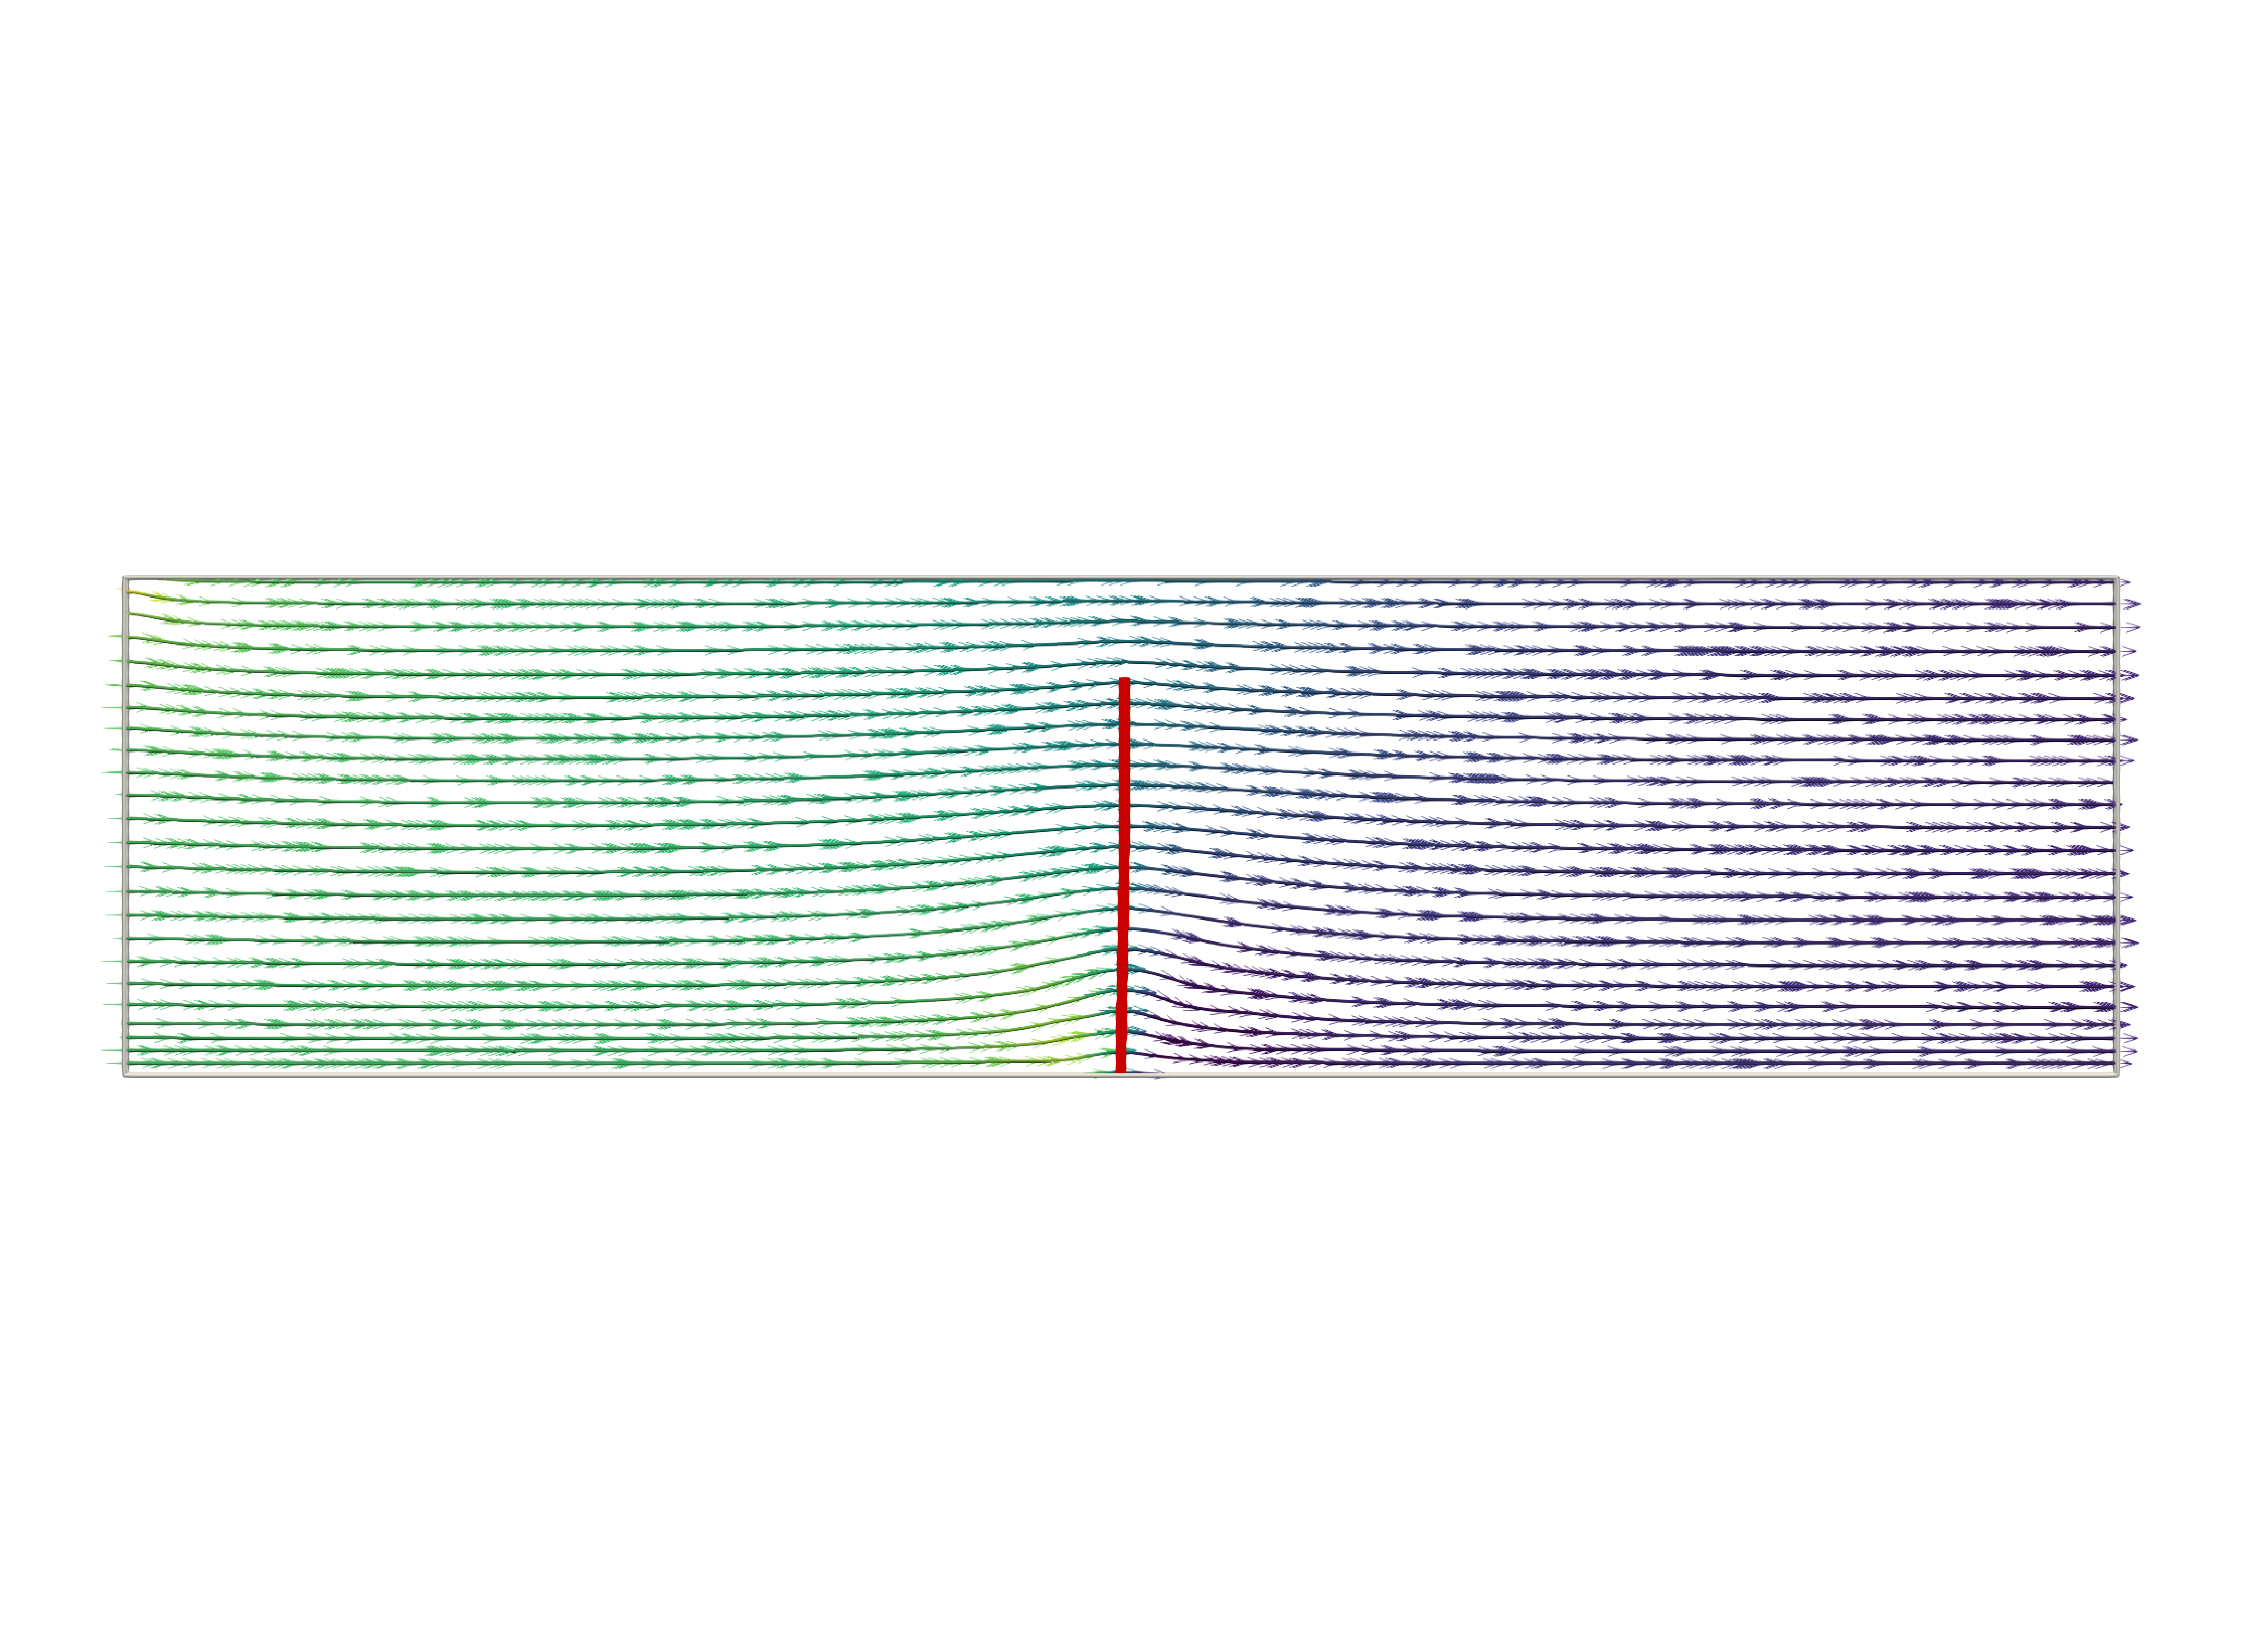
\includegraphics[width=\textwidth]{leaflet_snapshot_t0.pdf}
\caption{$t = 0$}
\end{subfigure}\hfill
\begin{subfigure}[b]{0.48\textwidth}
\centering
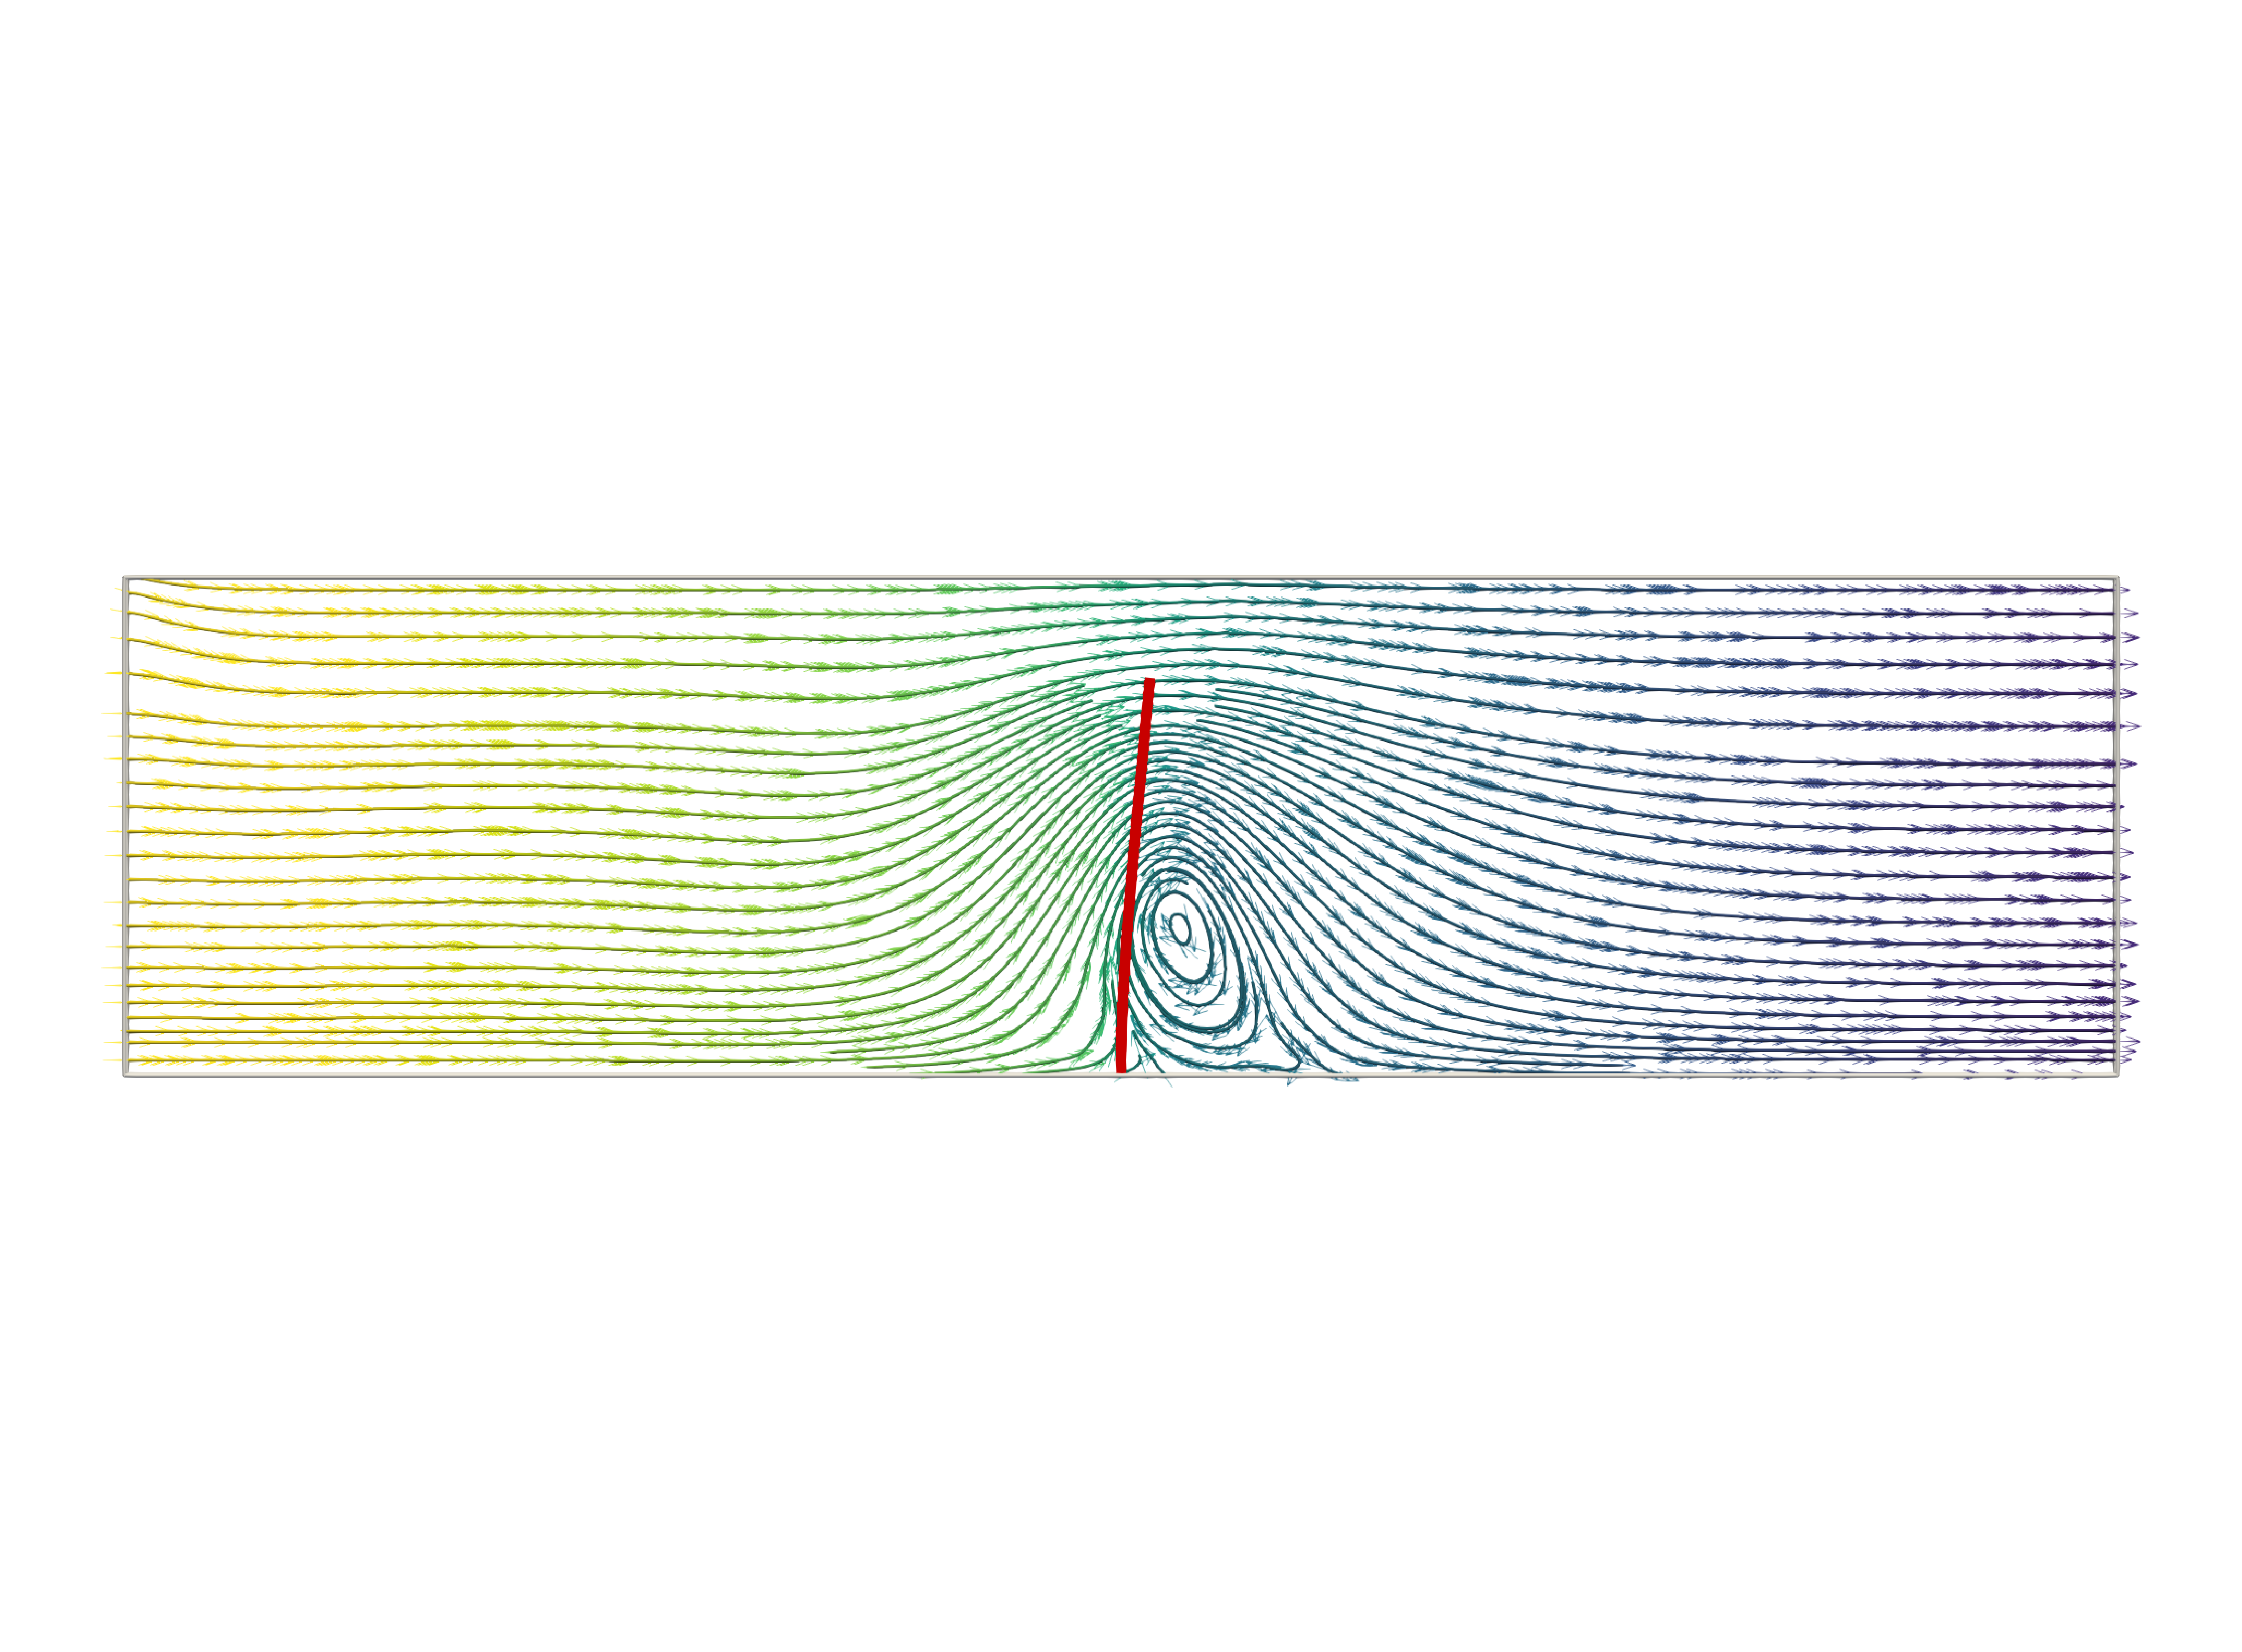
\includegraphics[width=\textwidth]{leaflet_snapshot_t1.pdf}
\caption{$t = T/8$}
\end{subfigure}\\[0.4em]
\begin{subfigure}[b]{0.48\textwidth}
\centering
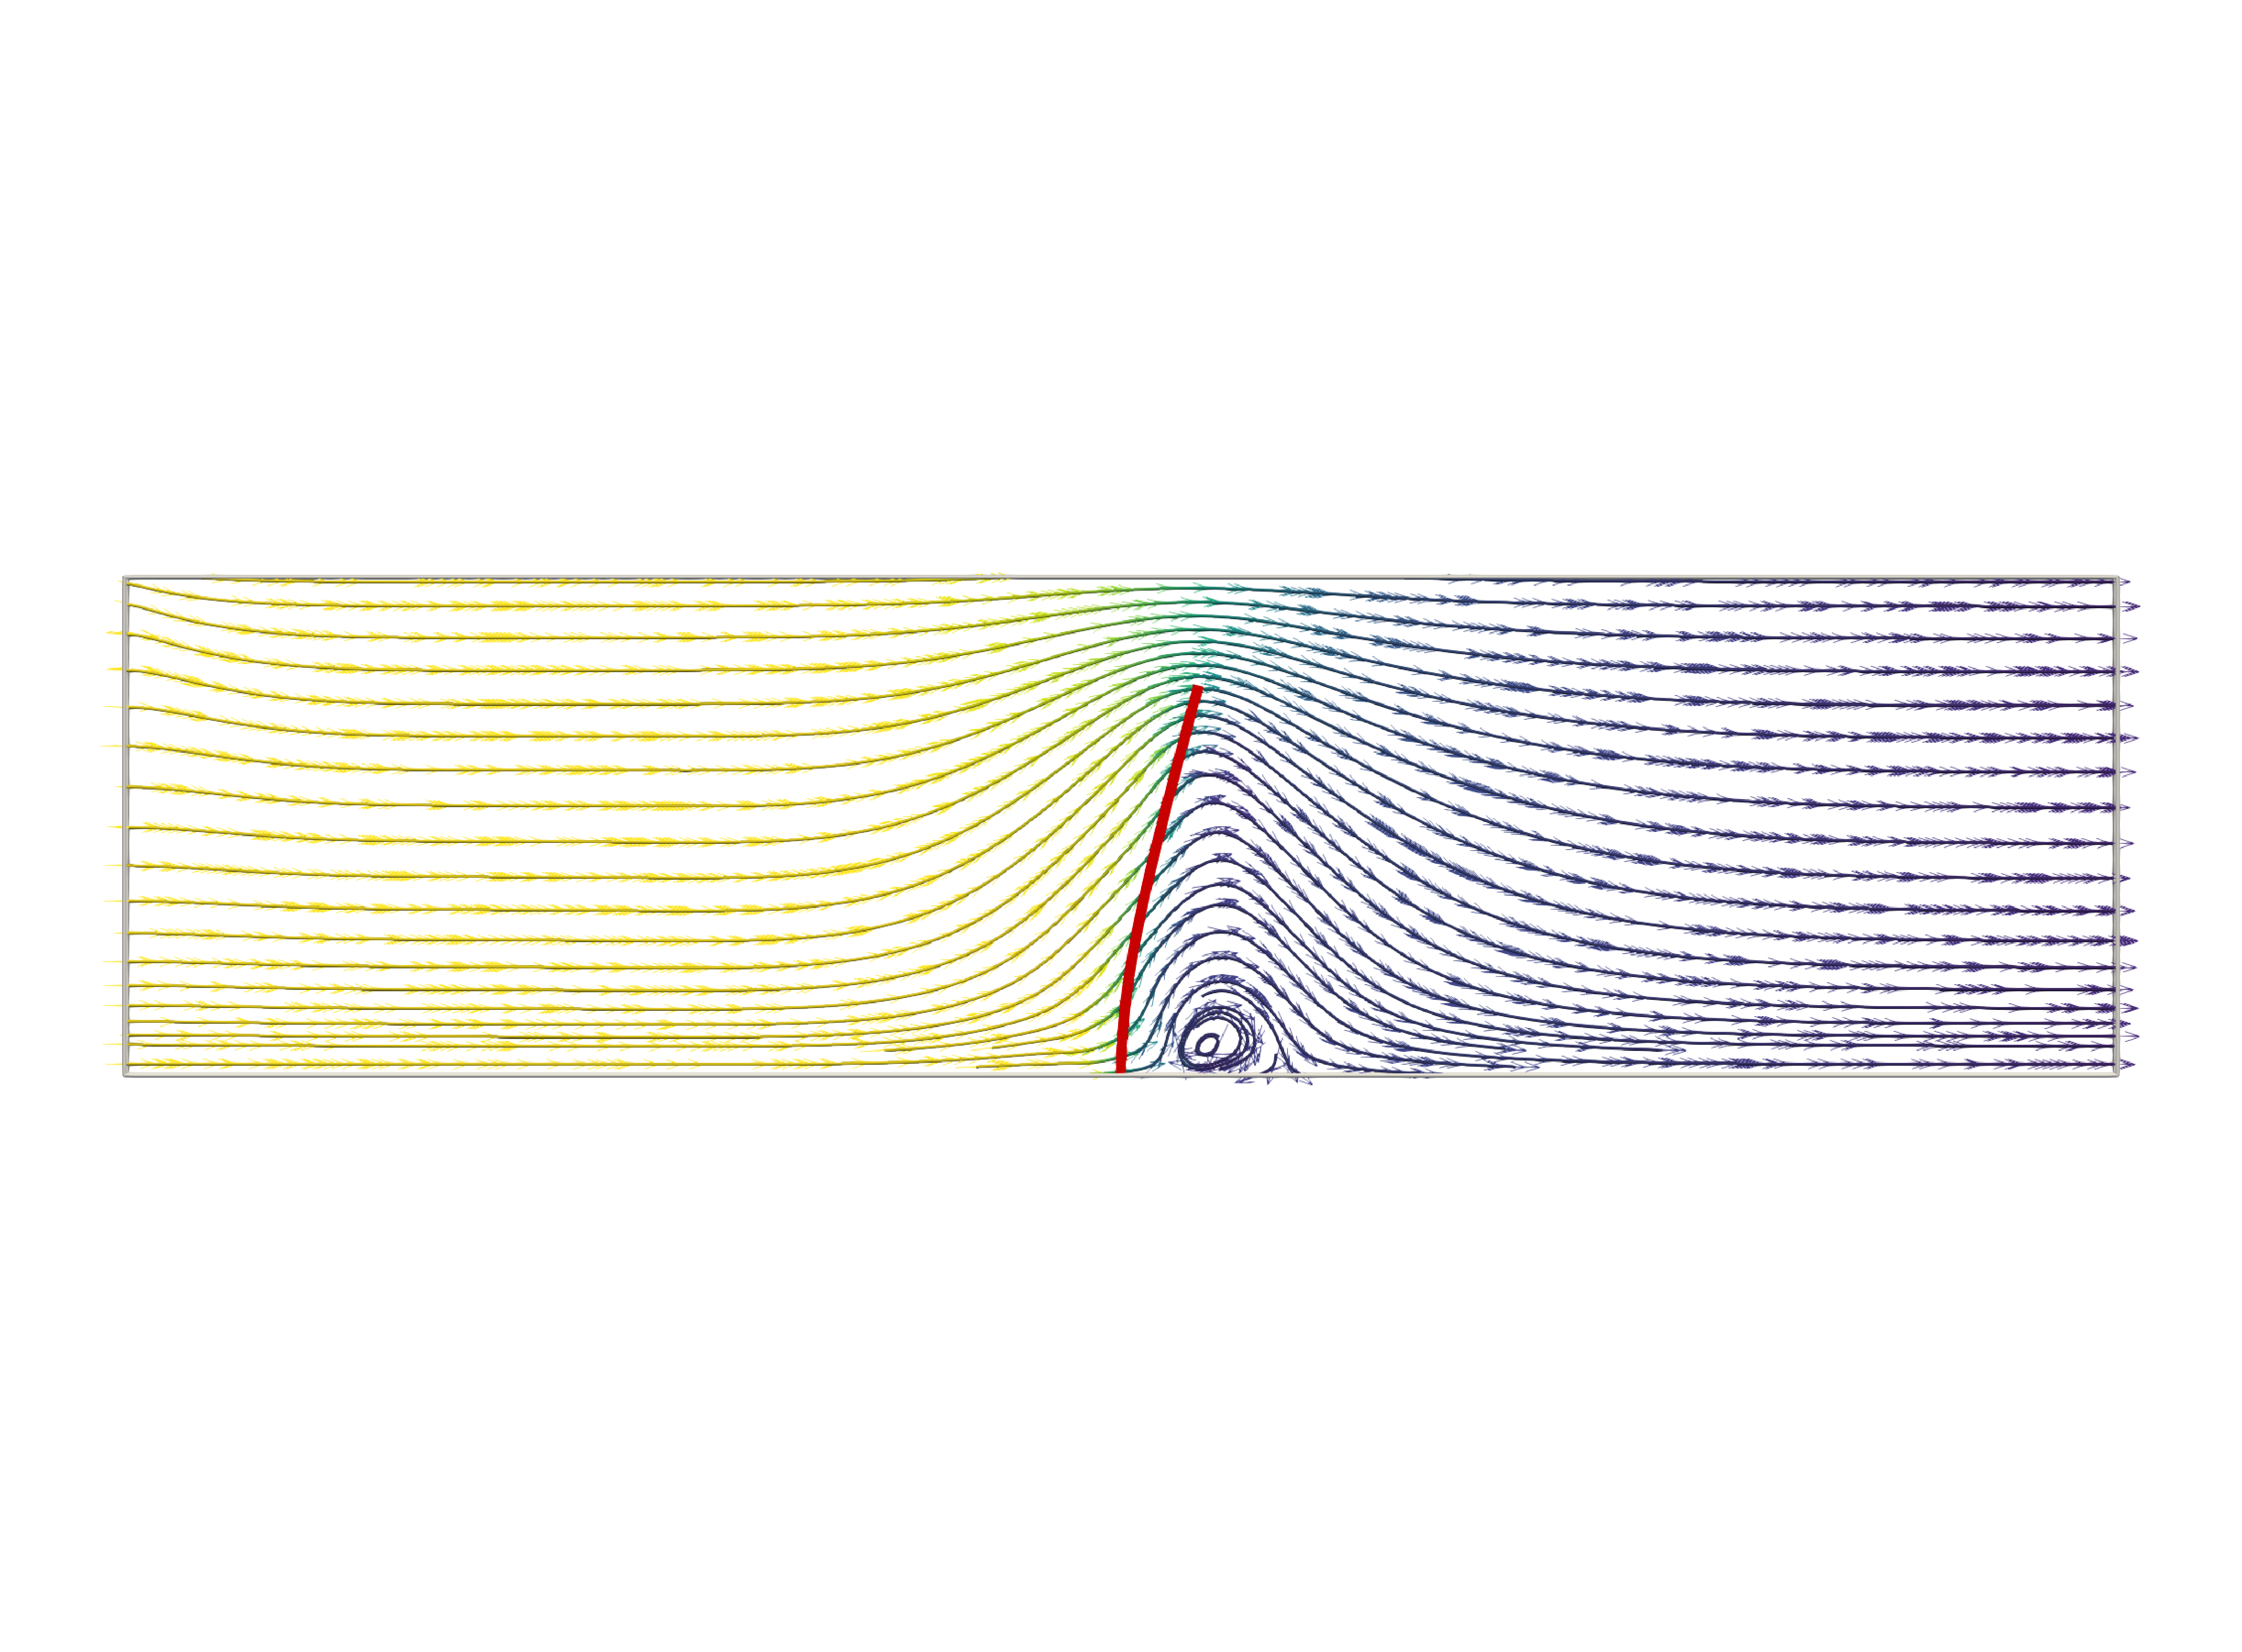
\includegraphics[width=\textwidth]{leaflet_snapshot_t2.pdf}
\caption{$t = T/4$}
\end{subfigure}\hfill
\begin{subfigure}[b]{0.48\textwidth}
\centering
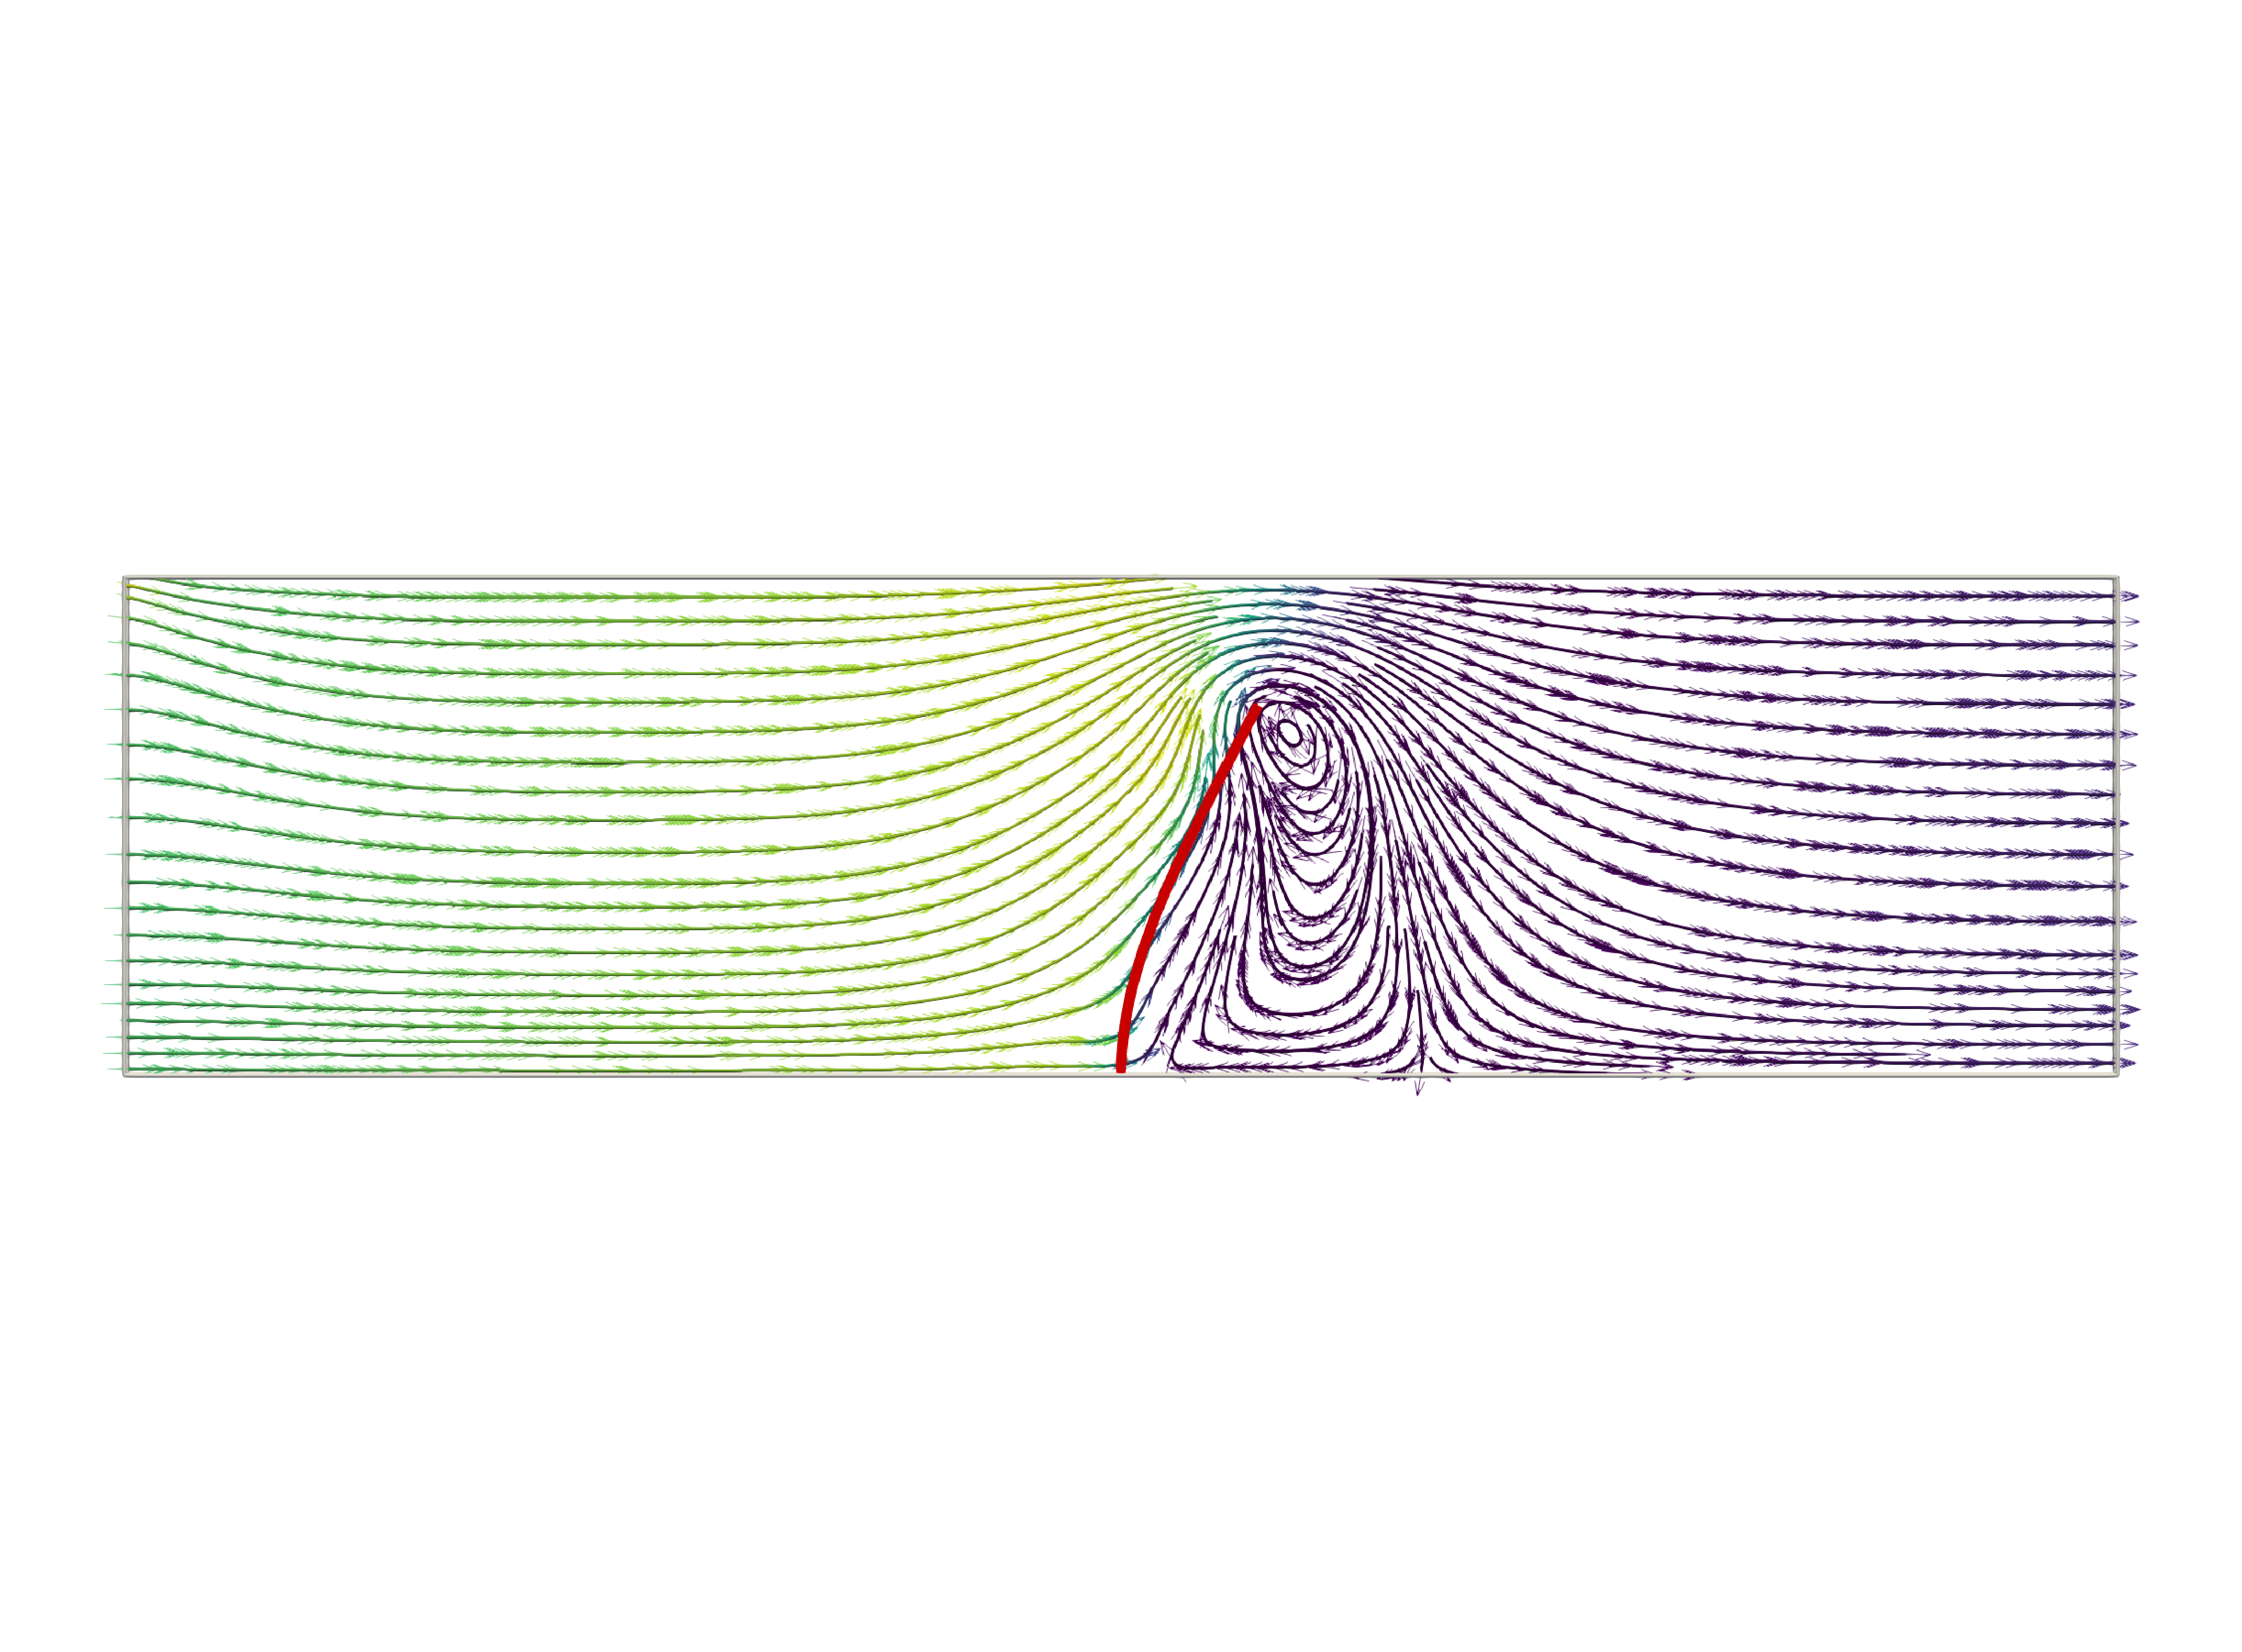
\includegraphics[width=\textwidth]{leaflet_snapshot_t3.pdf}
\caption{$t = 3T/8$}
\end{subfigure}\\[0.4em]
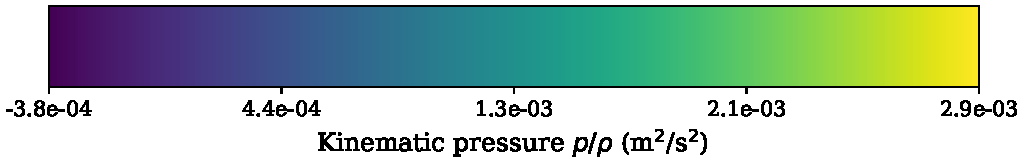
\includegraphics[width=0.80\textwidth]{leaflet_snapshots_cbar.pdf}
\caption{Mid-plane streamlines around the leaflet, coloured by kinematic pressure $p/\rho$ (shared colour bar below), over the first half of a converged forcing period of case C1 ($\mathrm{Re} = 10$, $\mathrm{St} = 1$, $T = 1~\mathrm{s}$), with the deflected actuator line overlaid in red. The second half of the period mirrors the first.}
\label{fig:leaflet_snapshots_panel}
\end{figure}

\noindent
Three features of these snapshots bear on the comparison with the reference in Section~\ref{sec:leaflet_results}. The absence of any small-scale vortex shedding throughout the period is consistent with the low cross-section Reynolds number of case C1 and supports the use of a $\mathrm{KC}$-independent drag coefficient. The tip excursion in the peak frame is visually consistent with the $\pm 2.324~\mathrm{mm}$ half-amplitude of the time-step study, which checks the integral trace at field level. The pressure dipole is generated entirely by the projected body force back-reacting on the fluid, so although the leaflet is geometrically absent from the mesh, its presence in the momentum equation produces the upstream-stagnation and downstream-suction structure that a body-fitted simulation would resolve at the plate surface, with the redistribution length set by the kernel width rather than by the plate thickness.

\subsection{Verification across the four (Re, St) cases}
\label{sec:leaflet_results}

\noindent
The coupled simulation is run at the four combinations of Table~\ref{tab:leaflet_cases}. All four runs share the same beam discretisation, fluid mesh, kernel width, and time step, and only the inlet amplitude, the forcing period, and the matching $C_{dn}$ vary. The reference traces are digitised from Figs.~13 and 14 of the reference paper.

\begin{figure}[!ht]
\centering
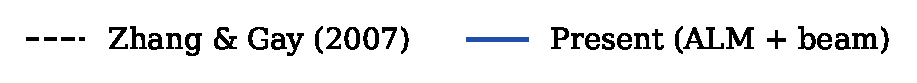
\includegraphics[width=0.90\textwidth]{leaflet_panel_legend.pdf}\\[0.3em]
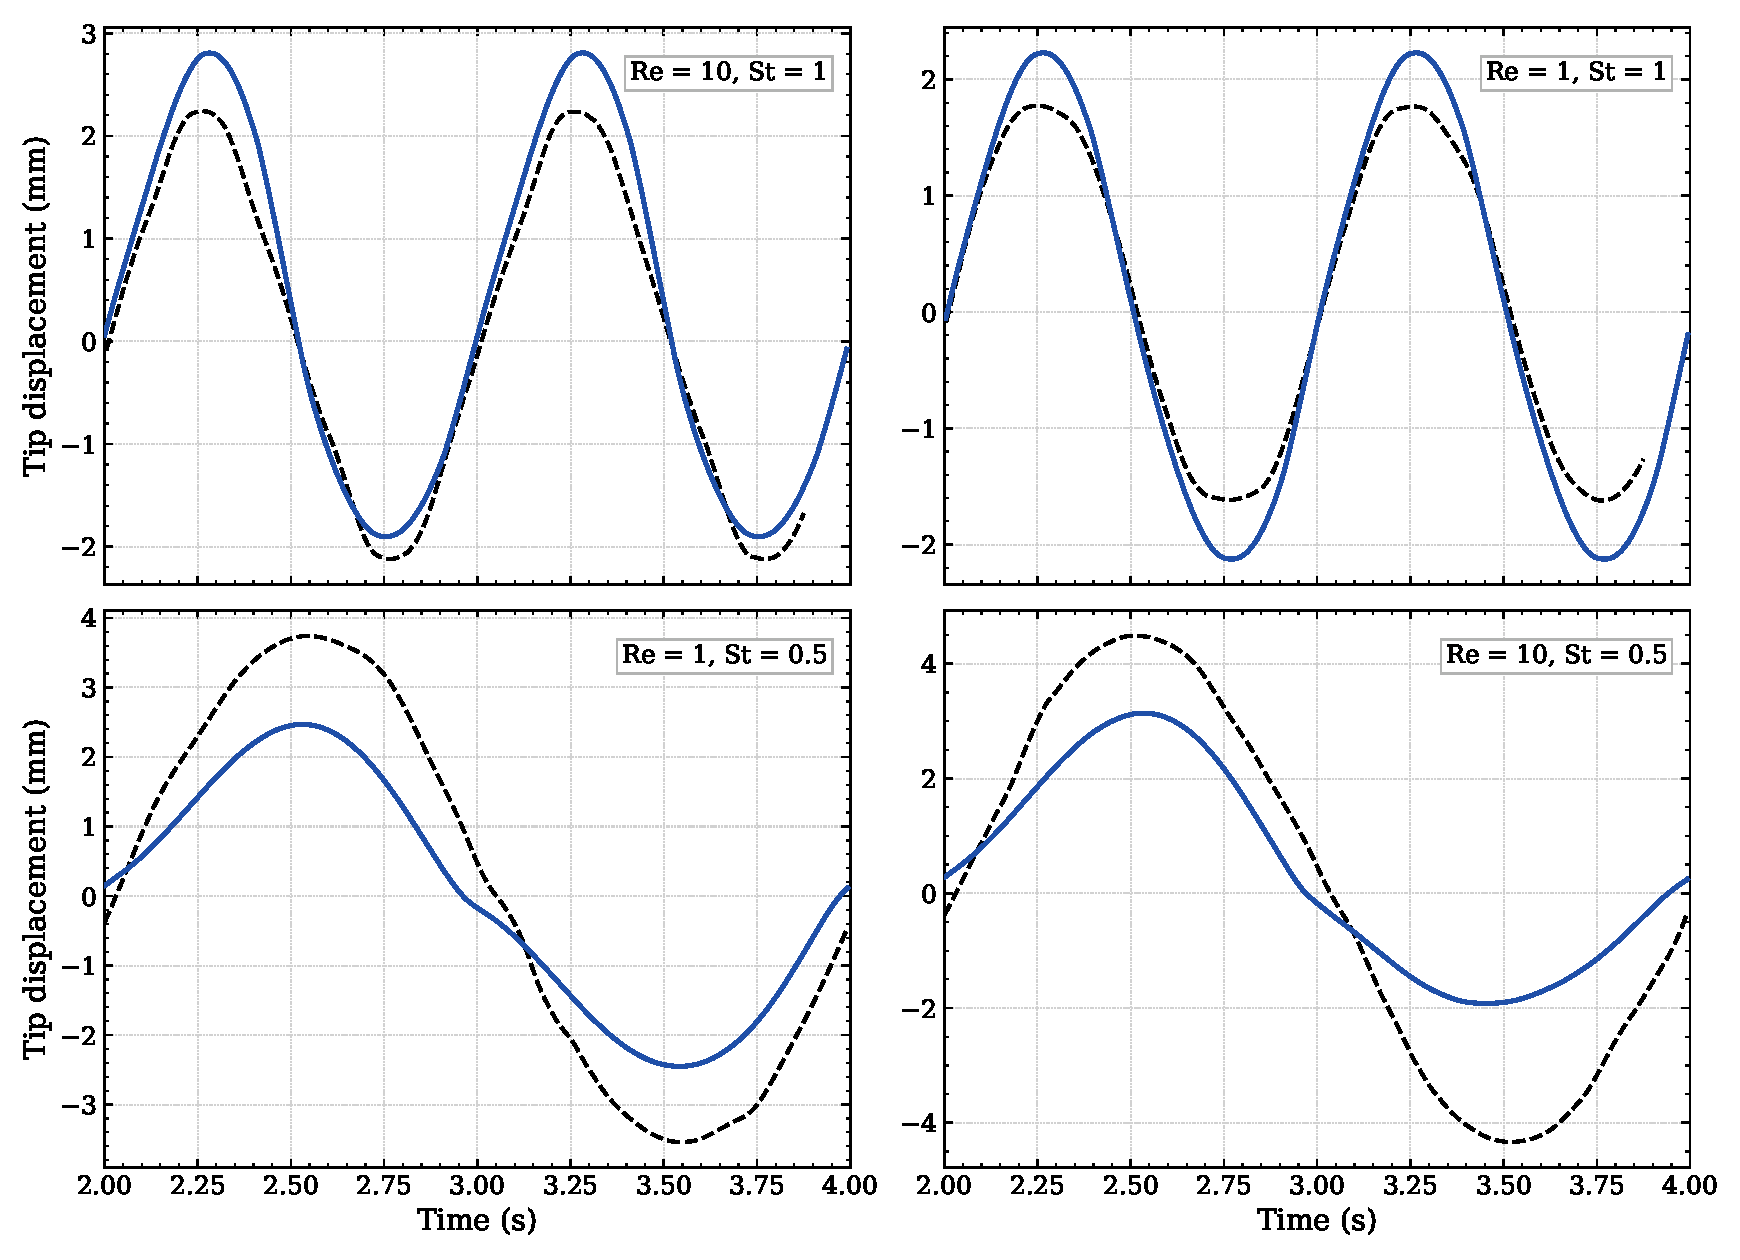
\includegraphics[width=\textwidth]{leaflet_panel.pdf}
\caption{Tip horizontal displacement traces for the four (Re, St) cases of \citet{zhang_immersed_2007}, Section~3.2. Dashed black lines are the digitised reference traces and solid blue lines the present result. Each trace has been phase-aligned to the reference by cross-correlation and windowed to the converged interval $t \in [2, 4]~\mathrm{s}$.}
\label{fig:leaflet_results_4cases}
\end{figure}

\noindent
Figure~\ref{fig:leaflet_results_4cases} compares the simulated tip displacement against the reference over the converged window. The agreement falls into two families. The cases at $\mathrm{St} = 1$ (C1 and C2) reproduce the reference period exactly and overshoot its peak excursion, the present values being $\pm 2.324~\mathrm{mm}$ against $\pm 2.2~\mathrm{mm}$ at C1 and $\pm 2.2~\mathrm{mm}$ against $\pm 1.7~\mathrm{mm}$ at C2, with the phase coinciding within plotting accuracy and the cycle-to-cycle shape closely matched. The cases at $\mathrm{St} = 0.5$ (C3 and C4) behave differently. The simulated peak excursion is essentially fixed near $\pm 2.5~\mathrm{mm}$, whereas the reference reaches $\pm 3.7~\mathrm{mm}$ at C3 and $\pm 4.5~\mathrm{mm}$ at C4, so the simulation under-predicts the reference peak excursion by $30\%$ in both cases. The period is again reproduced exactly, so the discrepancy is purely in amplitude.

\paragraph{Origin of the Strouhal-dependent discrepancy.}
The quasi-steady closure of Eq.~\eqref{eq:almLineForce} depends only on the instantaneous sampled velocity and carries no fluid-inertia term proportional to the acceleration, whereas in the IFEM reference the leaflet is immersed in a fully resolved Navier--Stokes field, so its force balance includes an added-mass term scaling with the local fluid acceleration and a history term depending on the past evolution of the relative motion. Halving the Strouhal number doubles the forcing period and halves the peak fluid acceleration at the inlet, and for a stationary member in an oscillating stream the classical Morison scaling would then predict the \emph{opposite} of the observed trend, since the ratio of inertia to drag scales as $1/\mathrm{KC}$ \citep{sarpkaya_mechanics_1981}. The growing under-prediction at $\mathrm{St} = 0.5$ must therefore originate in the unsteady forces associated with the leaflet's own motion, which the fixed-body scaling does not describe. At the longer period the reference excursion roughly doubles, so the relative acceleration between the leaflet and the surrounding fluid, and with it the added-mass reaction on the moving structure, remains dynamically significant even as the inlet acceleration halves, while at $\mathrm{Re}_{t} \approx 0.2$ the viscous history contribution depends on the past relative motion in a way that no instantaneous coefficient can represent. Apportioning the deficit among these terms would require a force decomposition of the reference solution, which the published data do not provide, so what the present results establish is the operational boundary of the closure rather than the split between the missing terms.

\noindent
One further observation supports this picture. The drag coefficient of the rigid plate is essentially independent of the Keulegan--Carpenter number in this regime, an unsteady re-run of the rigid-plate calibration at $\mathrm{KC} = 47$ and $94$ giving $C_{d} \approx 107$ in both. The textbook $C_{dn}(\mathrm{KC})$ trend that operates at higher Reynolds numbers does not apply at $\mathrm{Re}_{t} \approx 0.2$, where the wake remains attached and vortex shedding is suppressed. The Strouhal-dependent discrepancy is therefore not driven by a Strouhal-dependent drag coefficient on the rigid plate, but by the unsteady inertia of the surrounding fluid acting on the moving leaflet, which is the term that the classical Morison equation separates from the quadratic drag and that the present closure does not carry.

\noindent
The deterioration is documented quantitatively rather than removed by case-specific recalibration, since replacing the steady-CFD $C_{dn}$ with a per-case empirical value would mask the modelling limitation behind a parameter sweep. The framework is therefore verified over a clearly defined range of conditions, namely the drag-dominated regime represented here by the Strouhal number of $1$ rather than $0.5$, and extending it further would require an unsteady closure that adds explicit added-mass and history terms to Eq.~\eqref{eq:almLineForce}.

